\section{II. Luật chơi Saboteur}

% 1
\begin{frame}
\frametitle{Bộ bài Saboteur đầy đủ}

\begin{figure}[H]
    \centering
    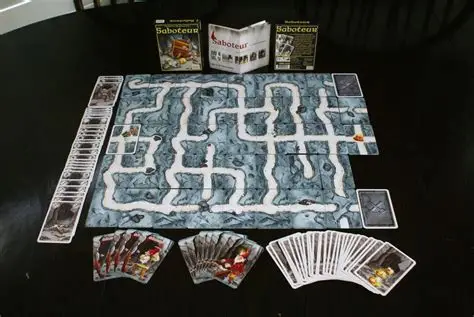
\includegraphics[width=0.6\linewidth]{luat_choi/image.png}
\end{figure}

\end{frame}

% 2
% \begin{frame}
% \frametitle{Tổng quan Saboteur}
% \begin{columns}
%     \column{0.5\textwidth}
%     \textbf{Tổng quan và mục tiêu}
%     \begin{itemize}
%         \item Số người chơi: 3--10.
%         \item Mục tiêu:
%         \begin{itemize}
%             \item \textbf{Gold-Diggers}: mở đường từ Start đến Goal chứa vàng.
%             \item \textbf{Saboteurs}: phá để Gold-Diggers không thể đến được vàng.
%         \end{itemize}
%     \end{itemize}

%     \column{0.5\textwidth}
%     \textbf{Trang bị trong bộ Saboteur}
%     \begin{itemize}
%         \item 40 Thẻ đường (path cards): gồm 31 thẻ thông, 9 thẻ cụt
%         \item 27 Thẻ hành động (action cards)
%         \item 11 Thẻ vai trò (role cards)
%     \end{itemize}
% \end{columns}
% \end{frame}

% % 3
% \begin{frame}
% \frametitle{Hình minh họa bộ thẻ và bàn chơi}

% \begin{figure}[H]
%     \centering
%     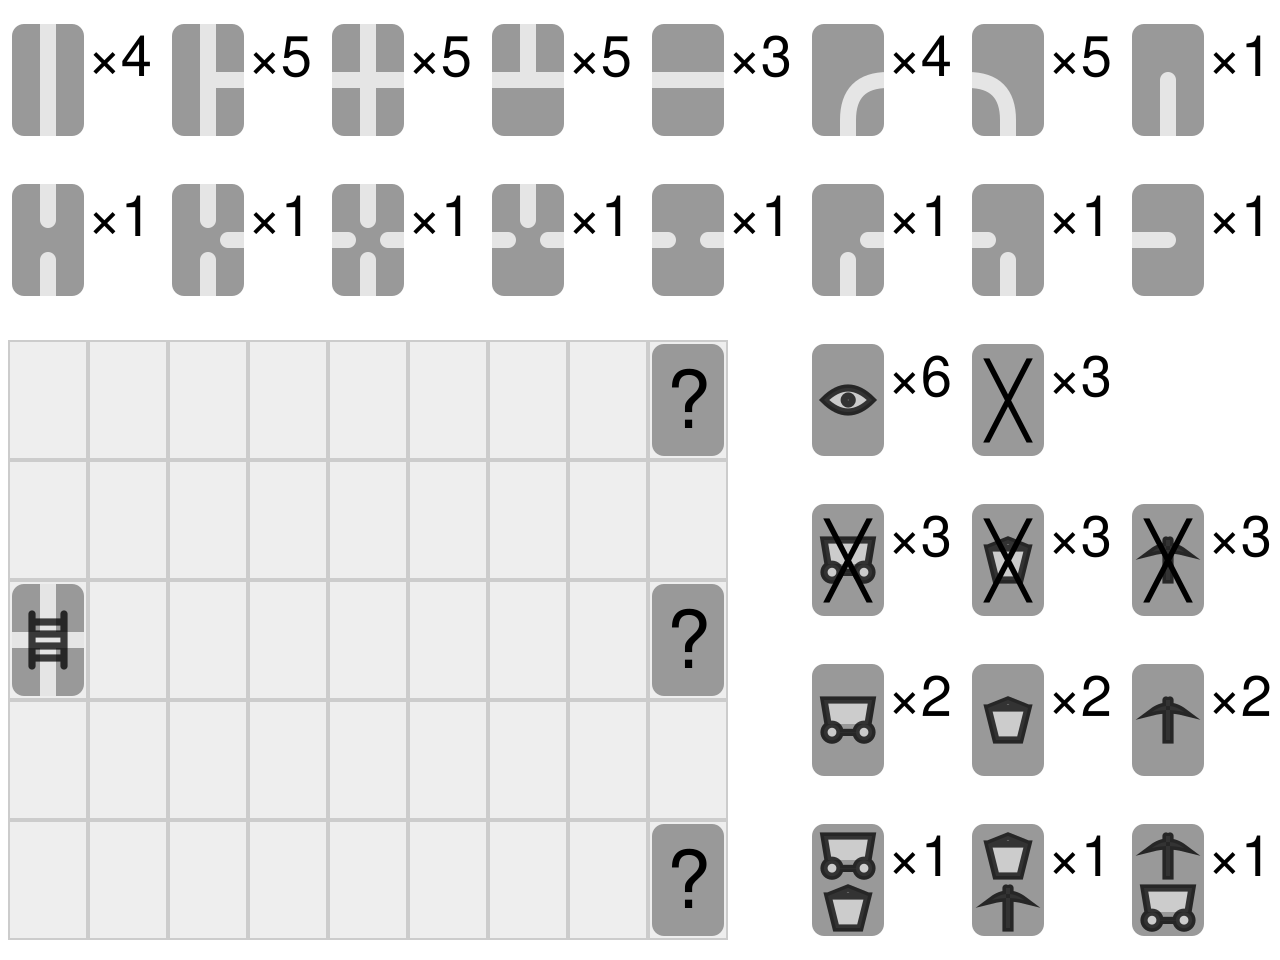
\includegraphics[width=0.6\linewidth]{luat_choi/saboteurCards.png}
%     \label{fig:cards-and-board}
% \end{figure}
% \end{frame}


\begin{frame}
\frametitle{Hai vai trò trong Saboteur}
\begin{columns}
    \column{0.5\textwidth}

    \begin{figure}[H]
        \centering
        
\includegraphics[width=0.3\linewidth]{saboteur/role-1.png}
    \end{figure}
    \textbf{Điều kiện thắng của Gold-Diggers:}
    
    Nối được đường thông từ Start đến 1 ô đích chứa vàng trước khi hết bài.

    \column{0.5\textwidth}
    \begin{figure}[H]
        \centering
        
\includegraphics[width=0.3\linewidth]{saboteur/role-2.png}
    \end{figure}
    \textbf{Điều kiện thắng của Saboteurs:} 
    
    Ngăn cản Gold-Diggers mở đường đến vàng cho đến khi hết bài.
\end{columns}
\vspace{1cm}
Vai trò được phát cho người chơi sẽ bị ẩn cho tới cuối game.
\end{frame}

% 4
\begin{frame}
\frametitle{Bố trí bàn chơi (Setup)}
    \begin{figure}[H]
        \centering
        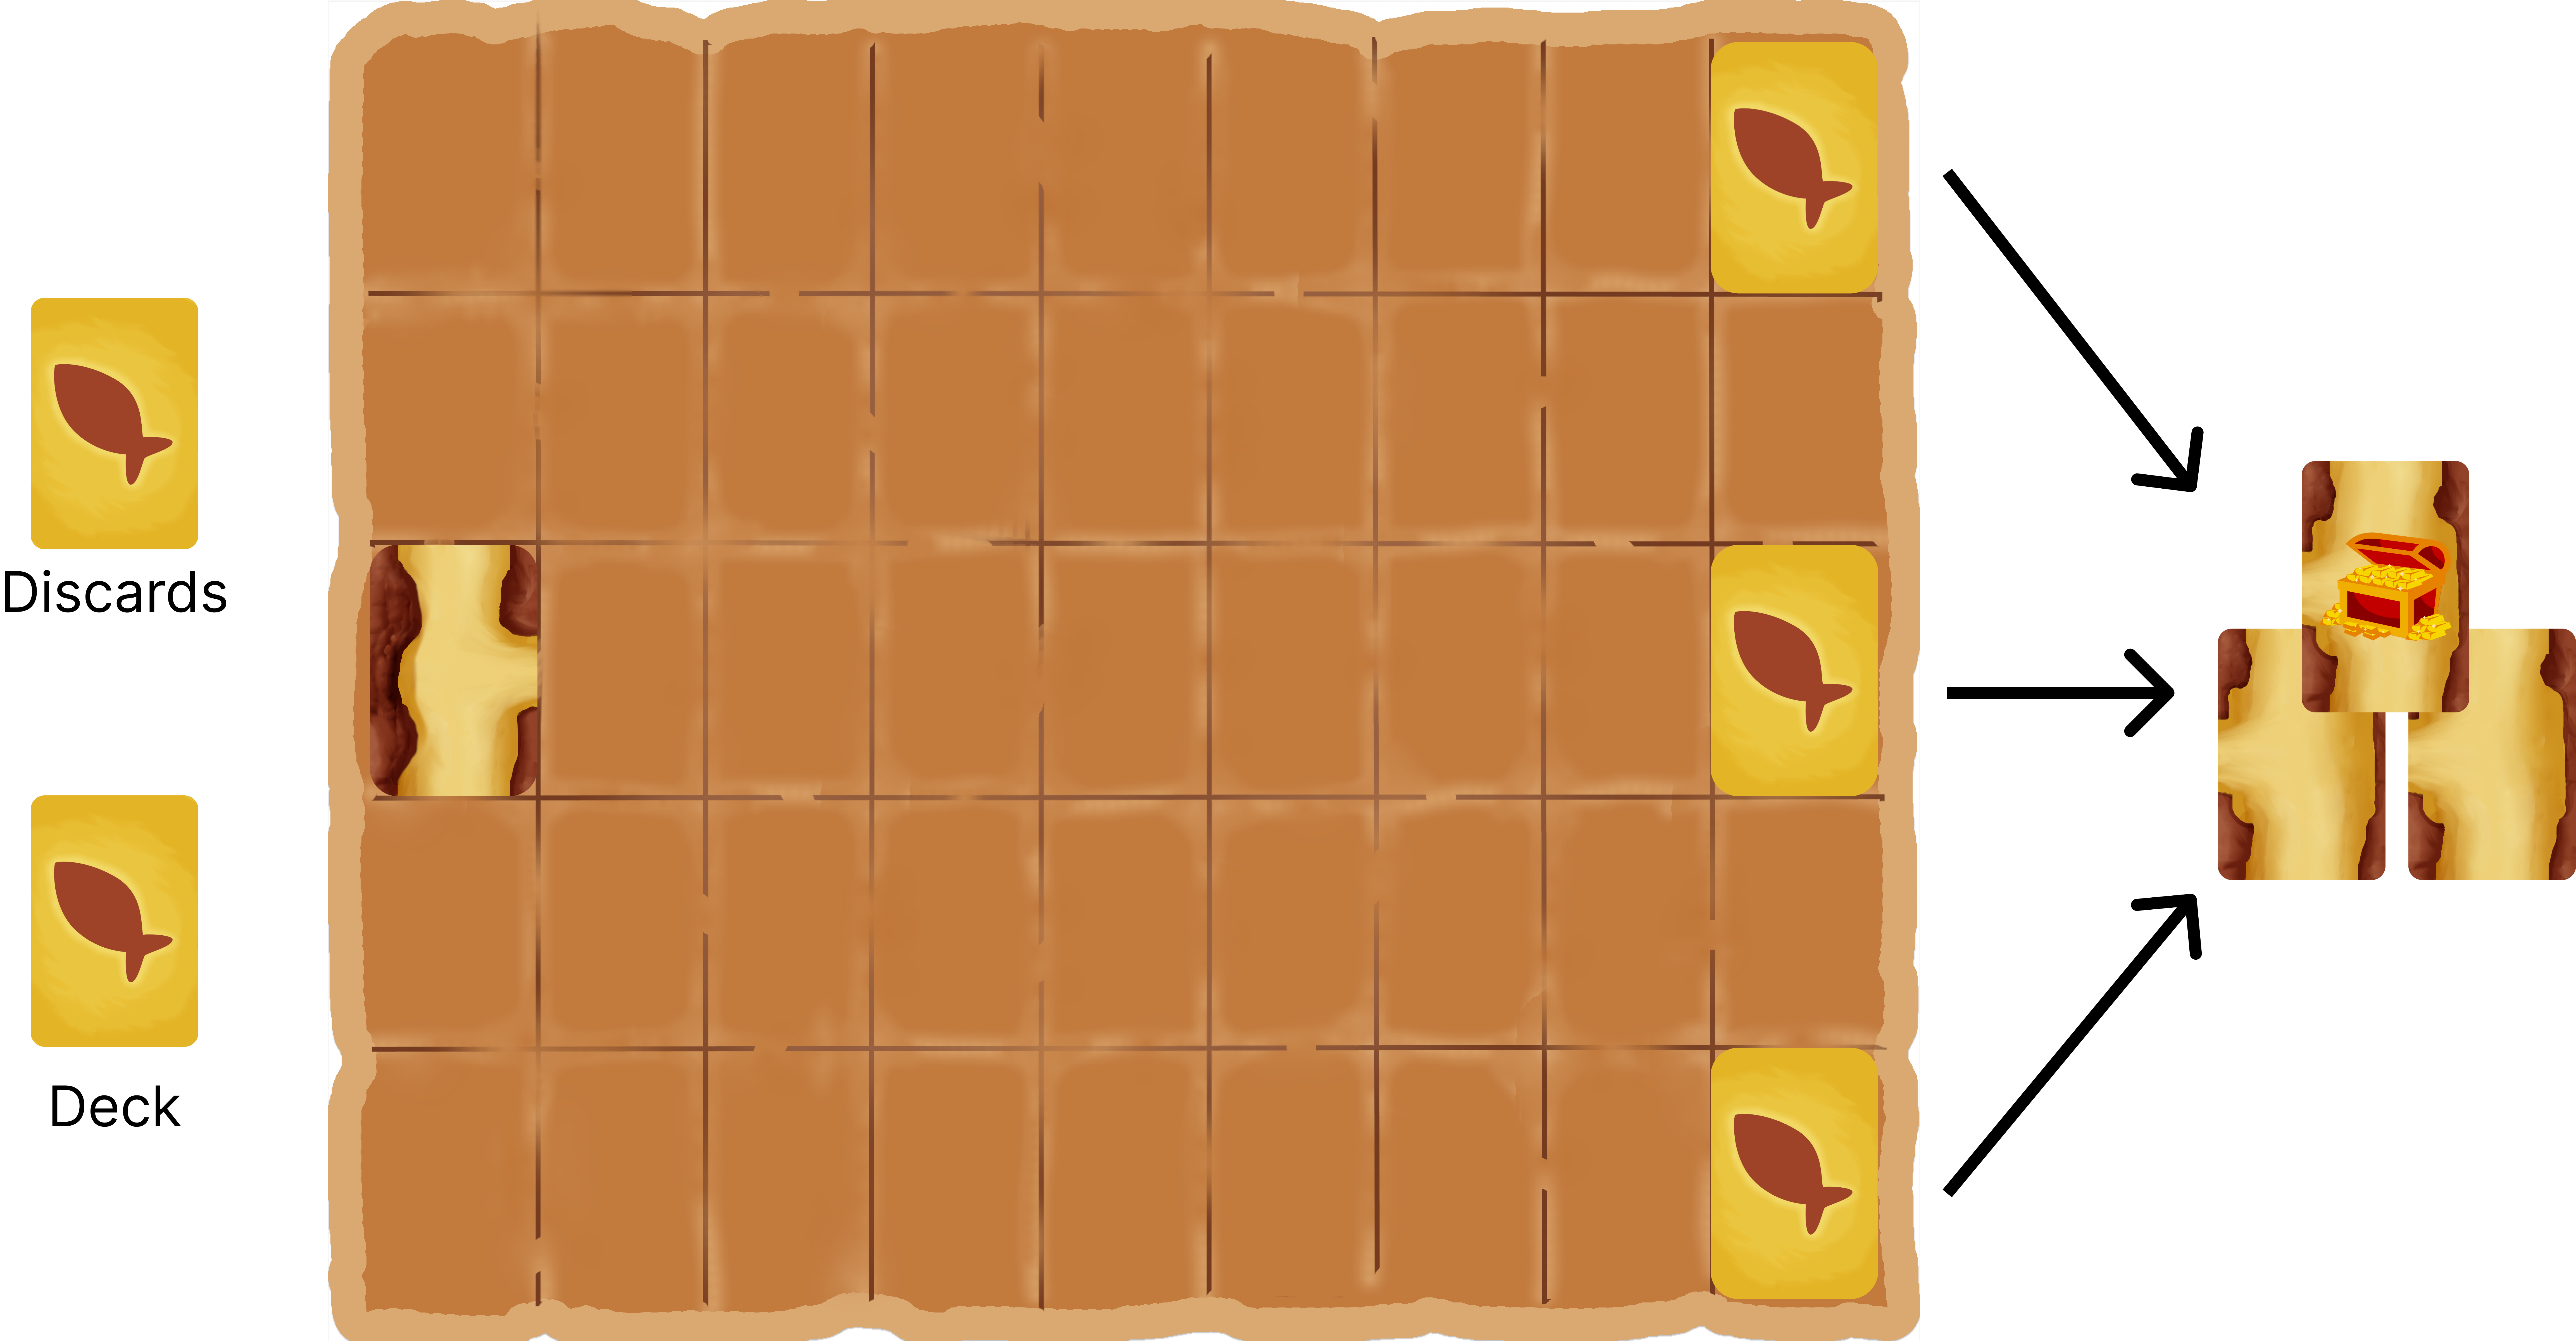
\includegraphics[width=0.8\linewidth]{saboteur/board2.png}
    \end{figure}
\end{frame}


% 5
\begin{frame}
\frametitle{Vòng chơi Saboteur}
\begin{columns}
    \column{0.5\textwidth}

    \begin{itemize}
    \item Lượt xoay chiều kim đồng hồ.
    \item Mỗi lượt chọn một trong các hành động:
    \begin{enumerate}
        \item Đặt thẻ đường (path card).
        \item Sử dụng thẻ hành động (action card).
        \item Bỏ thẻ (discard).
    \end{enumerate}
    \item Sau khi xong lượt của mình, người chơi bốc lên thẻ trên cùng của deck, lượt chơi tiếp tục qua người tiếp theo.
    \end{itemize}
\column{0.5\textwidth}
    \begin{figure}[H]
        \centering
        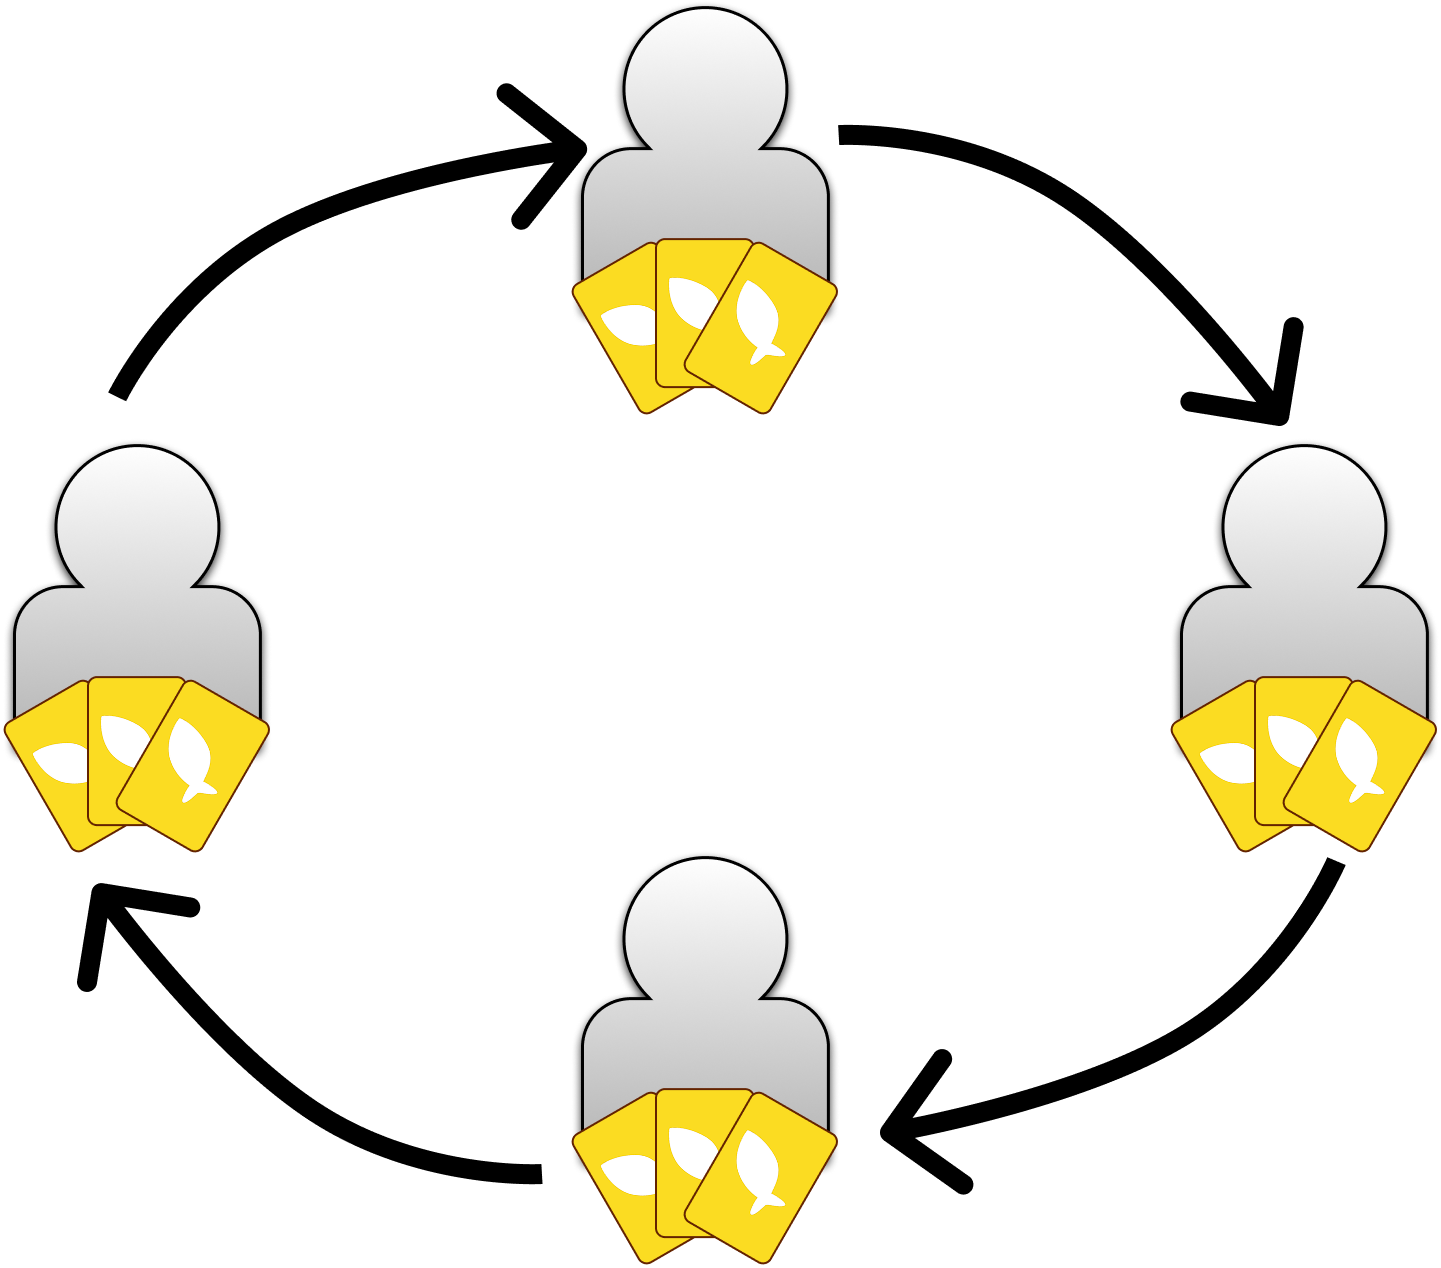
\includegraphics[width=0.5\linewidth]{saboteur/turn-cw.png}
        % \caption*{Các loại thẻ đường}
    \end{figure}
\end{columns}
\end{frame}

\begin{frame}
\frametitle{Vòng chơi Saboteur}
\begin{columns}
    \column{0.5\textwidth}

    \begin{itemize}
    \item Lượt xoay chiều kim đồng hồ.
    \item Mỗi lượt chọn một trong các hành động:
    \begin{enumerate}
        \item Đặt thẻ đường (path card).
        \item Sử dụng thẻ hành động (action card).
        \item Bỏ thẻ (discard).
    \end{enumerate}
    \item Sau khi xong lượt của mình, người chơi bốc lên thẻ trên cùng của deck, lượt chơi tiếp tục qua người tiếp theo.
    \end{itemize}
\column{0.5\textwidth}
    \begin{figure}[H]
        \centering
        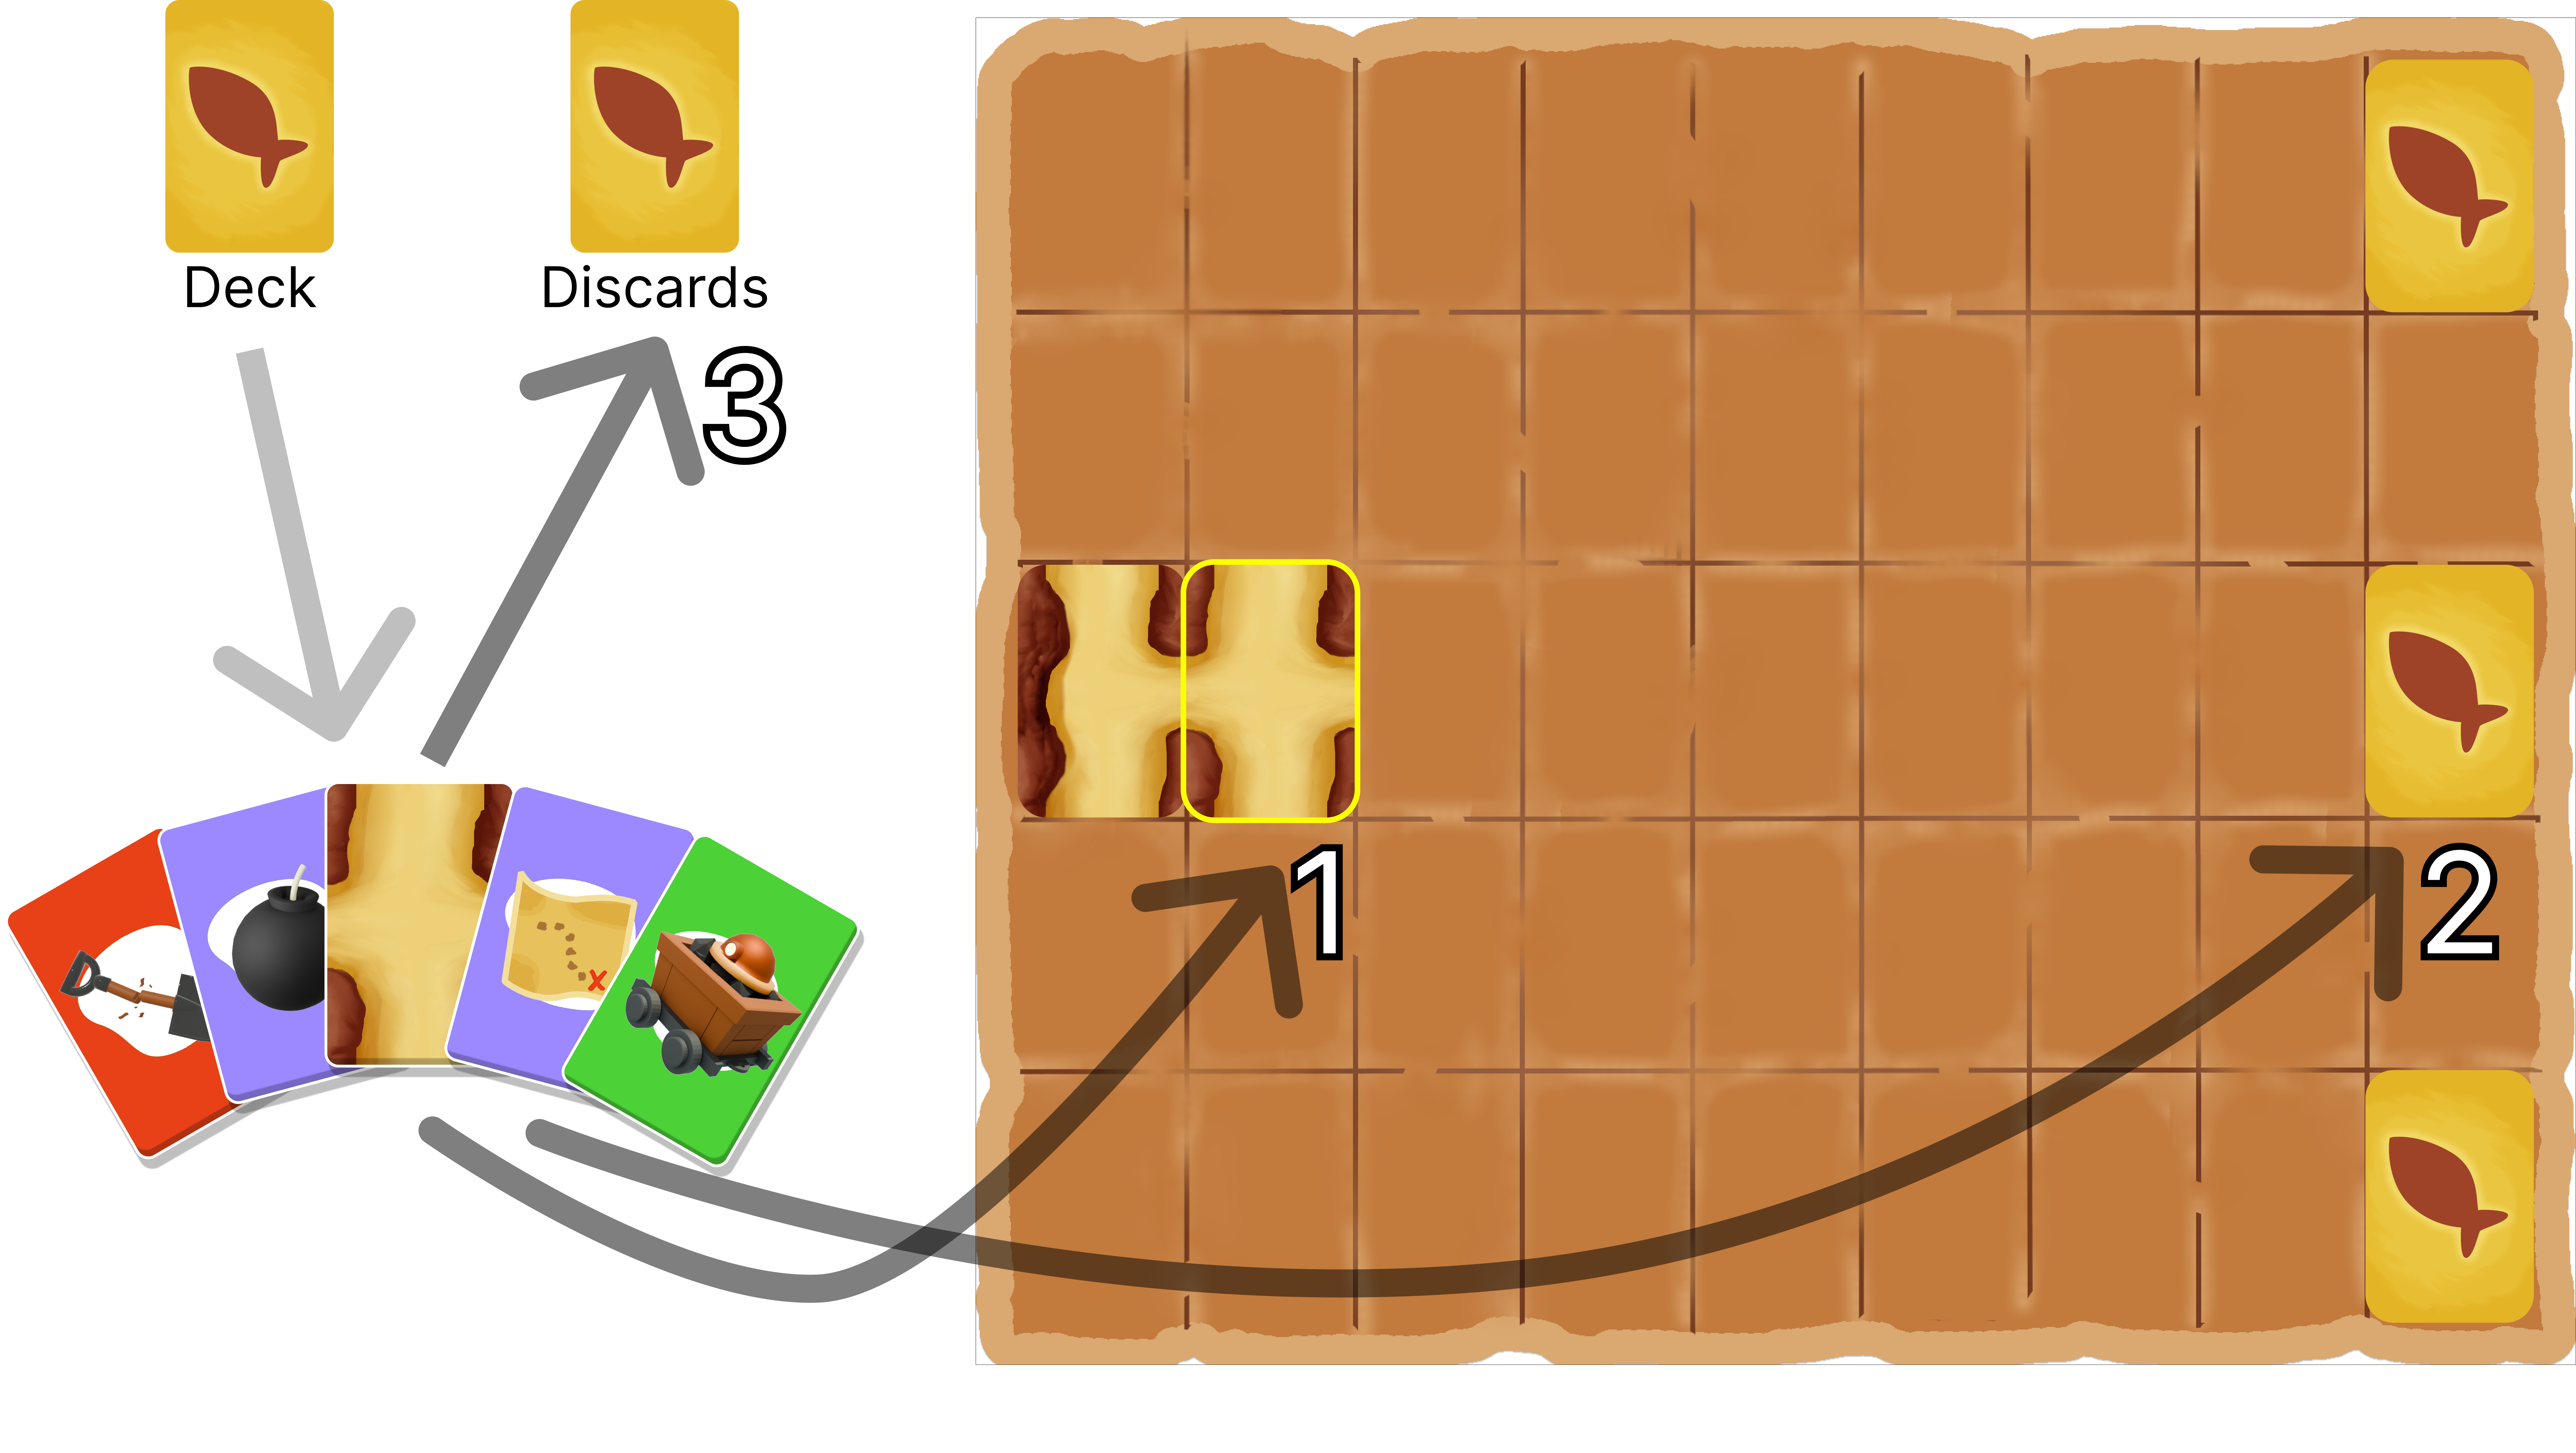
\includegraphics[width=0.8\linewidth]{saboteur/player-choices.png}
        % \caption*{Các loại thẻ đường}
    \end{figure}
\end{columns}
\end{frame}

% 6
\begin{frame}
\frametitle{Thẻ đường (Path Cards)}
    \vspace{1cm}
    \begin{figure}[H]
        \centering
        \includegraphics[width=0.8\linewidth]{saboteur/path-cards.png}
        \caption*{Các loại thẻ đường}
    \end{figure}
\end{frame}


\begin{frame}
\frametitle{Thẻ đường (Path Cards)}
    \vspace{1cm}
    \begin{figure}[H]
        \centering
        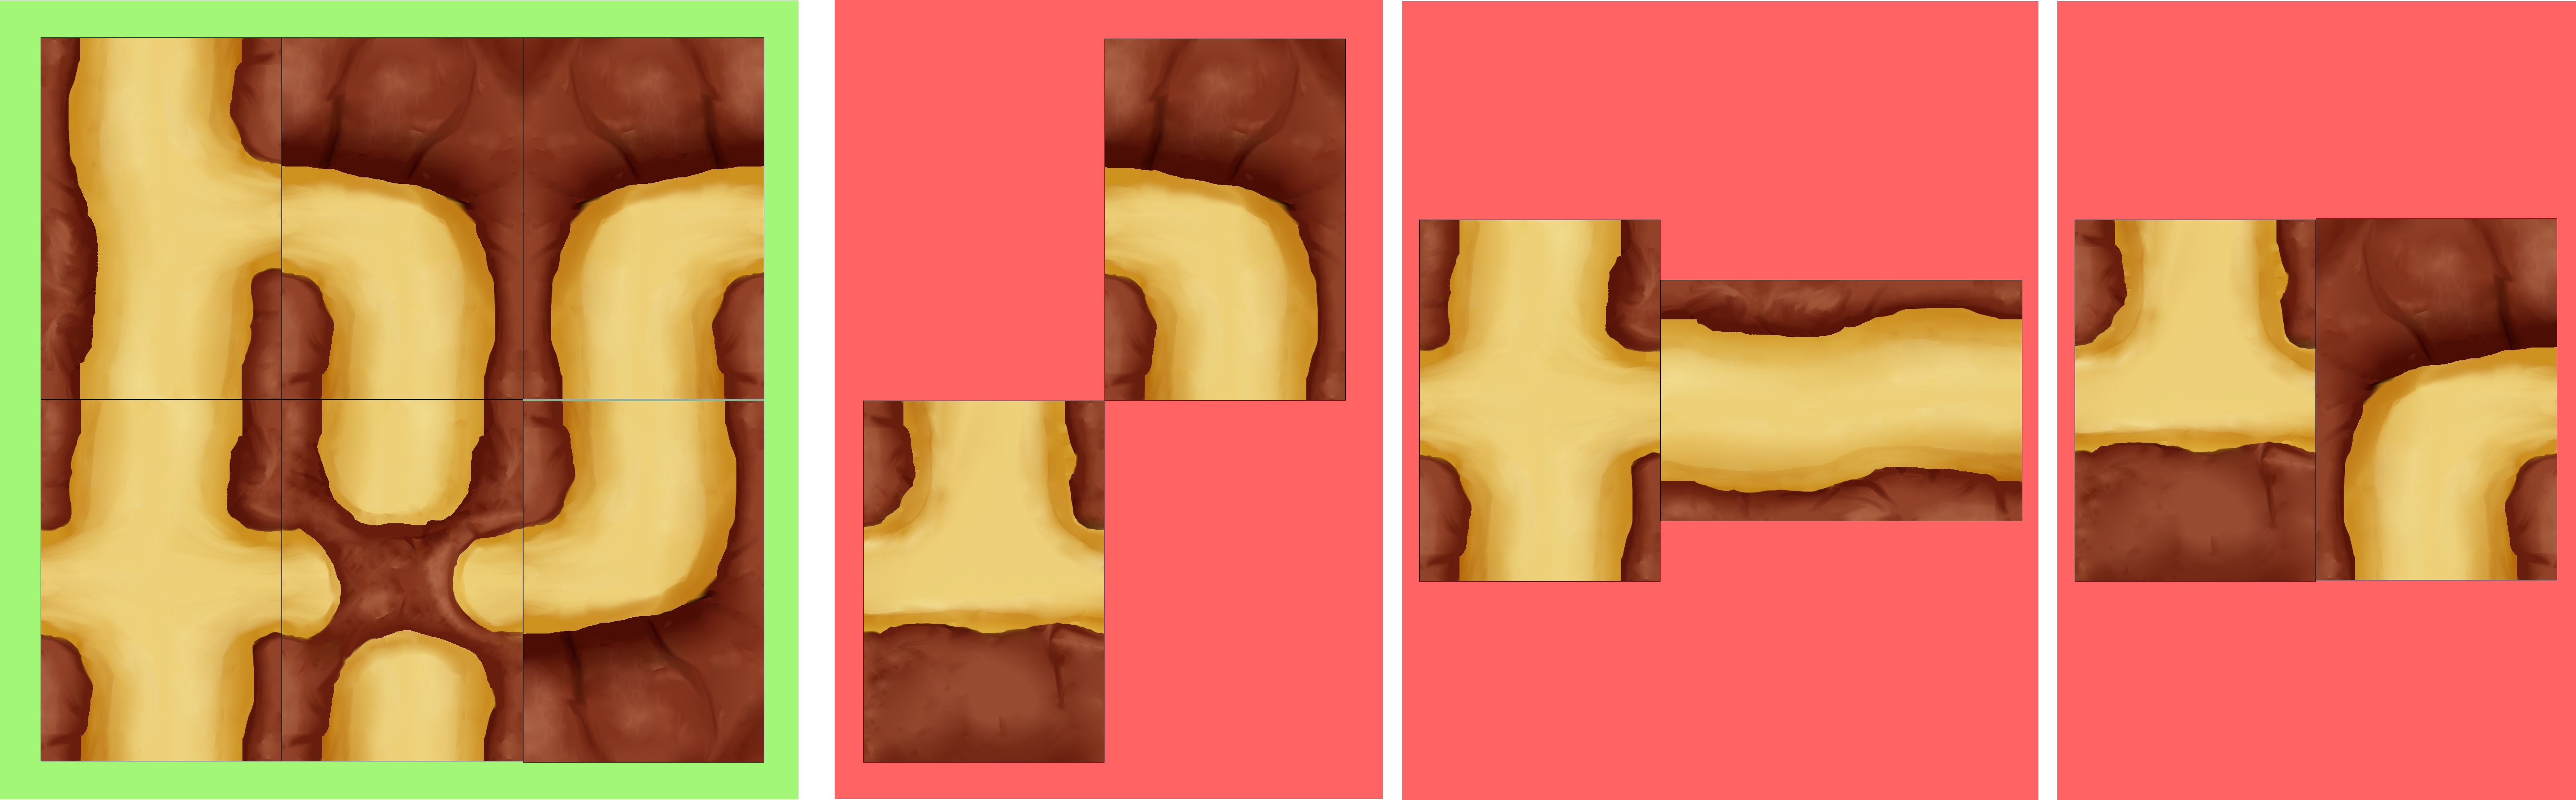
\includegraphics[width=0.8\linewidth]{saboteur/path-cards-placement.png}
        \caption*{Các trường hợp đặt thẻ đường}
    \end{figure}
\end{frame}

% 10
\begin{frame}
\frametitle{Thẻ hành động (Action Cards)}

    \begin{table}[H]
    \centering
    \begin{tabular}{|c|p{7cm}|c|}
    \hline
    \textbf{Loại thẻ} & \textbf{Công dụng} & \textbf{Số lượng} \\ \hline
    Sabotage & Phá 1 công cụ: Cart, Shovel hoặc Hat. Người bị phá không thể đặt Path cho đến khi được sửa. & 9 \\ \hline
    Repair   & Sửa công cụ bị phá. Gồm: 6 thẻ đơn (mỗi loại công cụ 2 thẻ), 3 thẻ kép. & 9 \\ \hline
    Map      & Cho phép xem lén 1 trong 3 thẻ Goal. Không được tiết lộ thông tin trừ khi tự nguyện. & 6 \\ \hline
    Bomb & Phá hủy 1 Path card trên bàn (trừ Start và 3 Goal). Thẻ bị phá được loại khỏi mỏ. & 3 \\ \hline
    \end{tabular}
    \end{table}
\end{frame}



\begin{frame}
\frametitle{Thẻ hành động (Action Cards)}
    \begin{figure}[H]
        \centering
        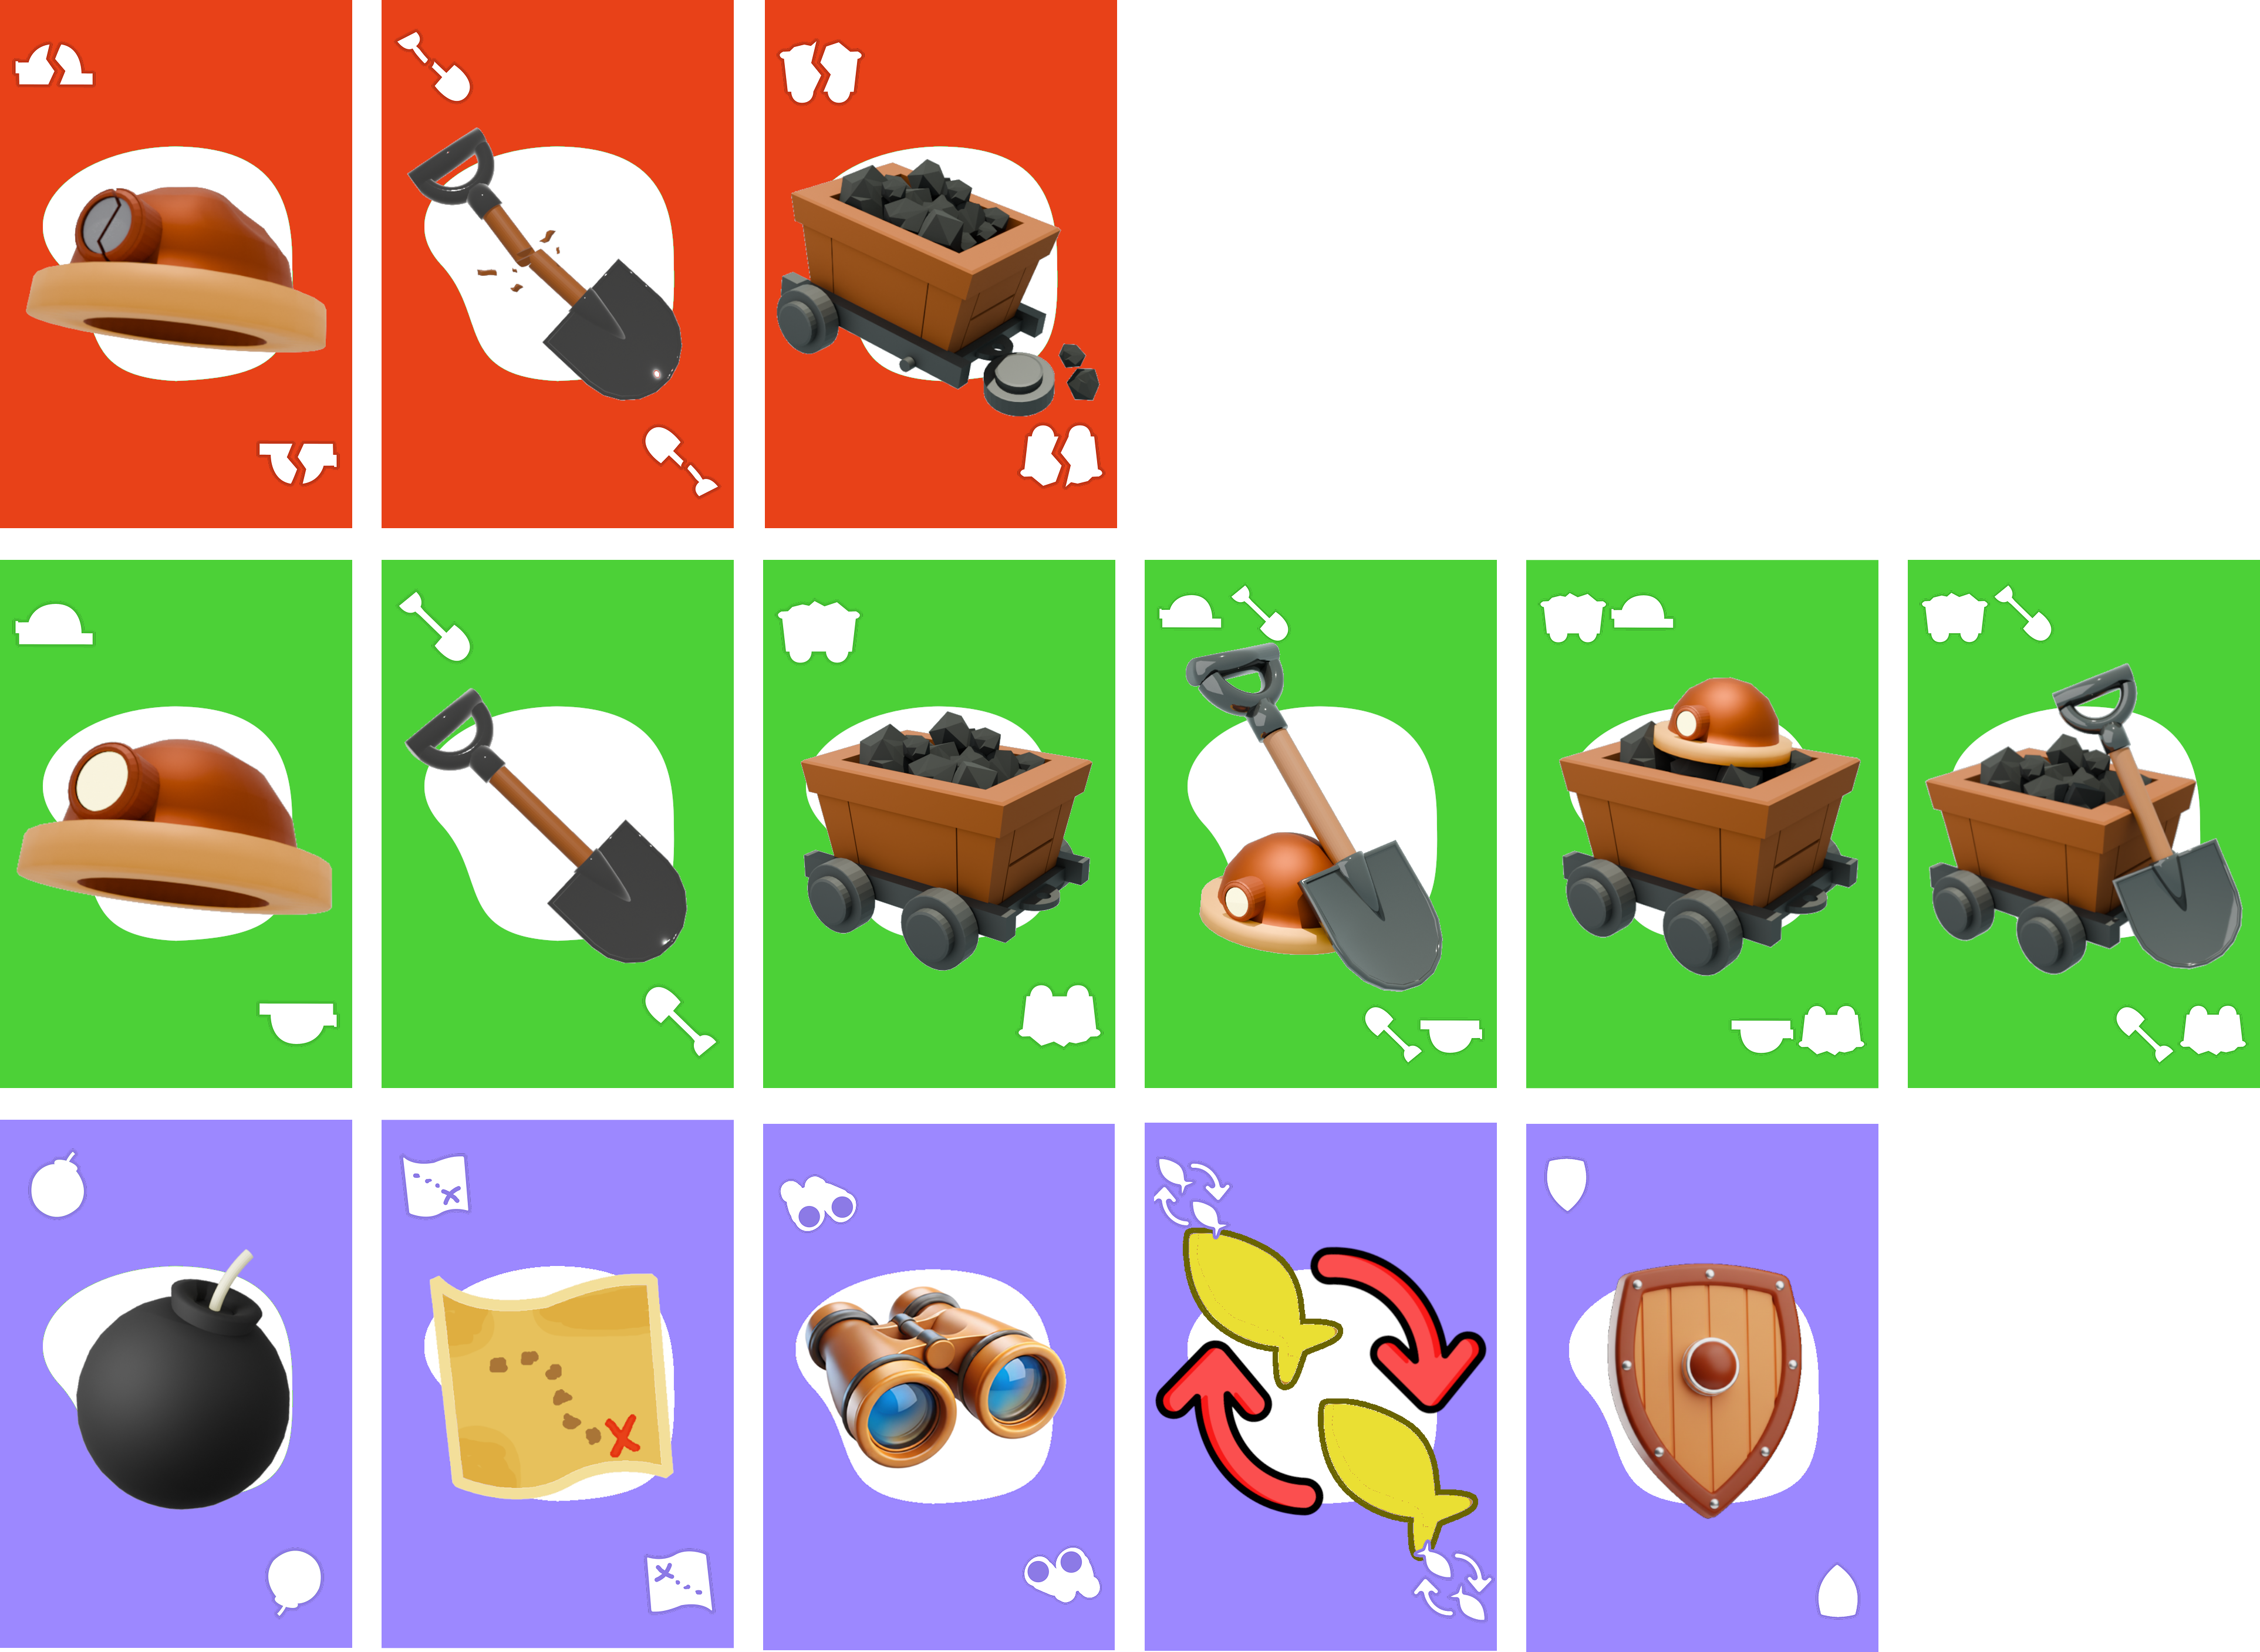
\includegraphics[width=0.6\linewidth]{saboteur/action-cards.png}
        \caption*{Các loại thẻ hành động}
    \end{figure}
\end{frame}

\begin{frame}
\frametitle{Thẻ hành động (Action Cards)}

\begin{columns}
    \column{0.5\textwidth}
    
    Các thẻ hành động ảnh hưởng trực tiếp đến khả năng đặt thẻ đường hoặc quan sát thông tin trong ván chơi.  
    Trong game có \textbf{3 loại công cụ}: 
    \begin{itemize}
        \item Xe đẩy (\textit{Cart})
        \item Xẻng (\textit{Shovel})
        \item Mũ (\textit{Hat})
    \end{itemize}

    \column{0.5\textwidth}
    Nếu người chơi bị phá \textbf{bất kỳ một trong ba công cụ}, họ \textbf{không thể đặt thẻ đường}.  
    Để sửa, người chơi phải dùng thẻ Repair tương ứng.

    \begin{itemize}
        \item \textbf{Repair đơn}: sửa đúng 1 công cụ được chỉ định trên thẻ.
        \item \textbf{Repair kép}: sửa 1 trong 2 công cụ hiển thị trên thẻ (Có biến thể có thể sửa cả hai đồng thời).
    \end{itemize}
\end{columns}
\end{frame}

\begin{frame}
\frametitle{Thẻ hành động (Action Cards)}
    \vspace{1cm}
    \begin{figure}[H]
        \centering
        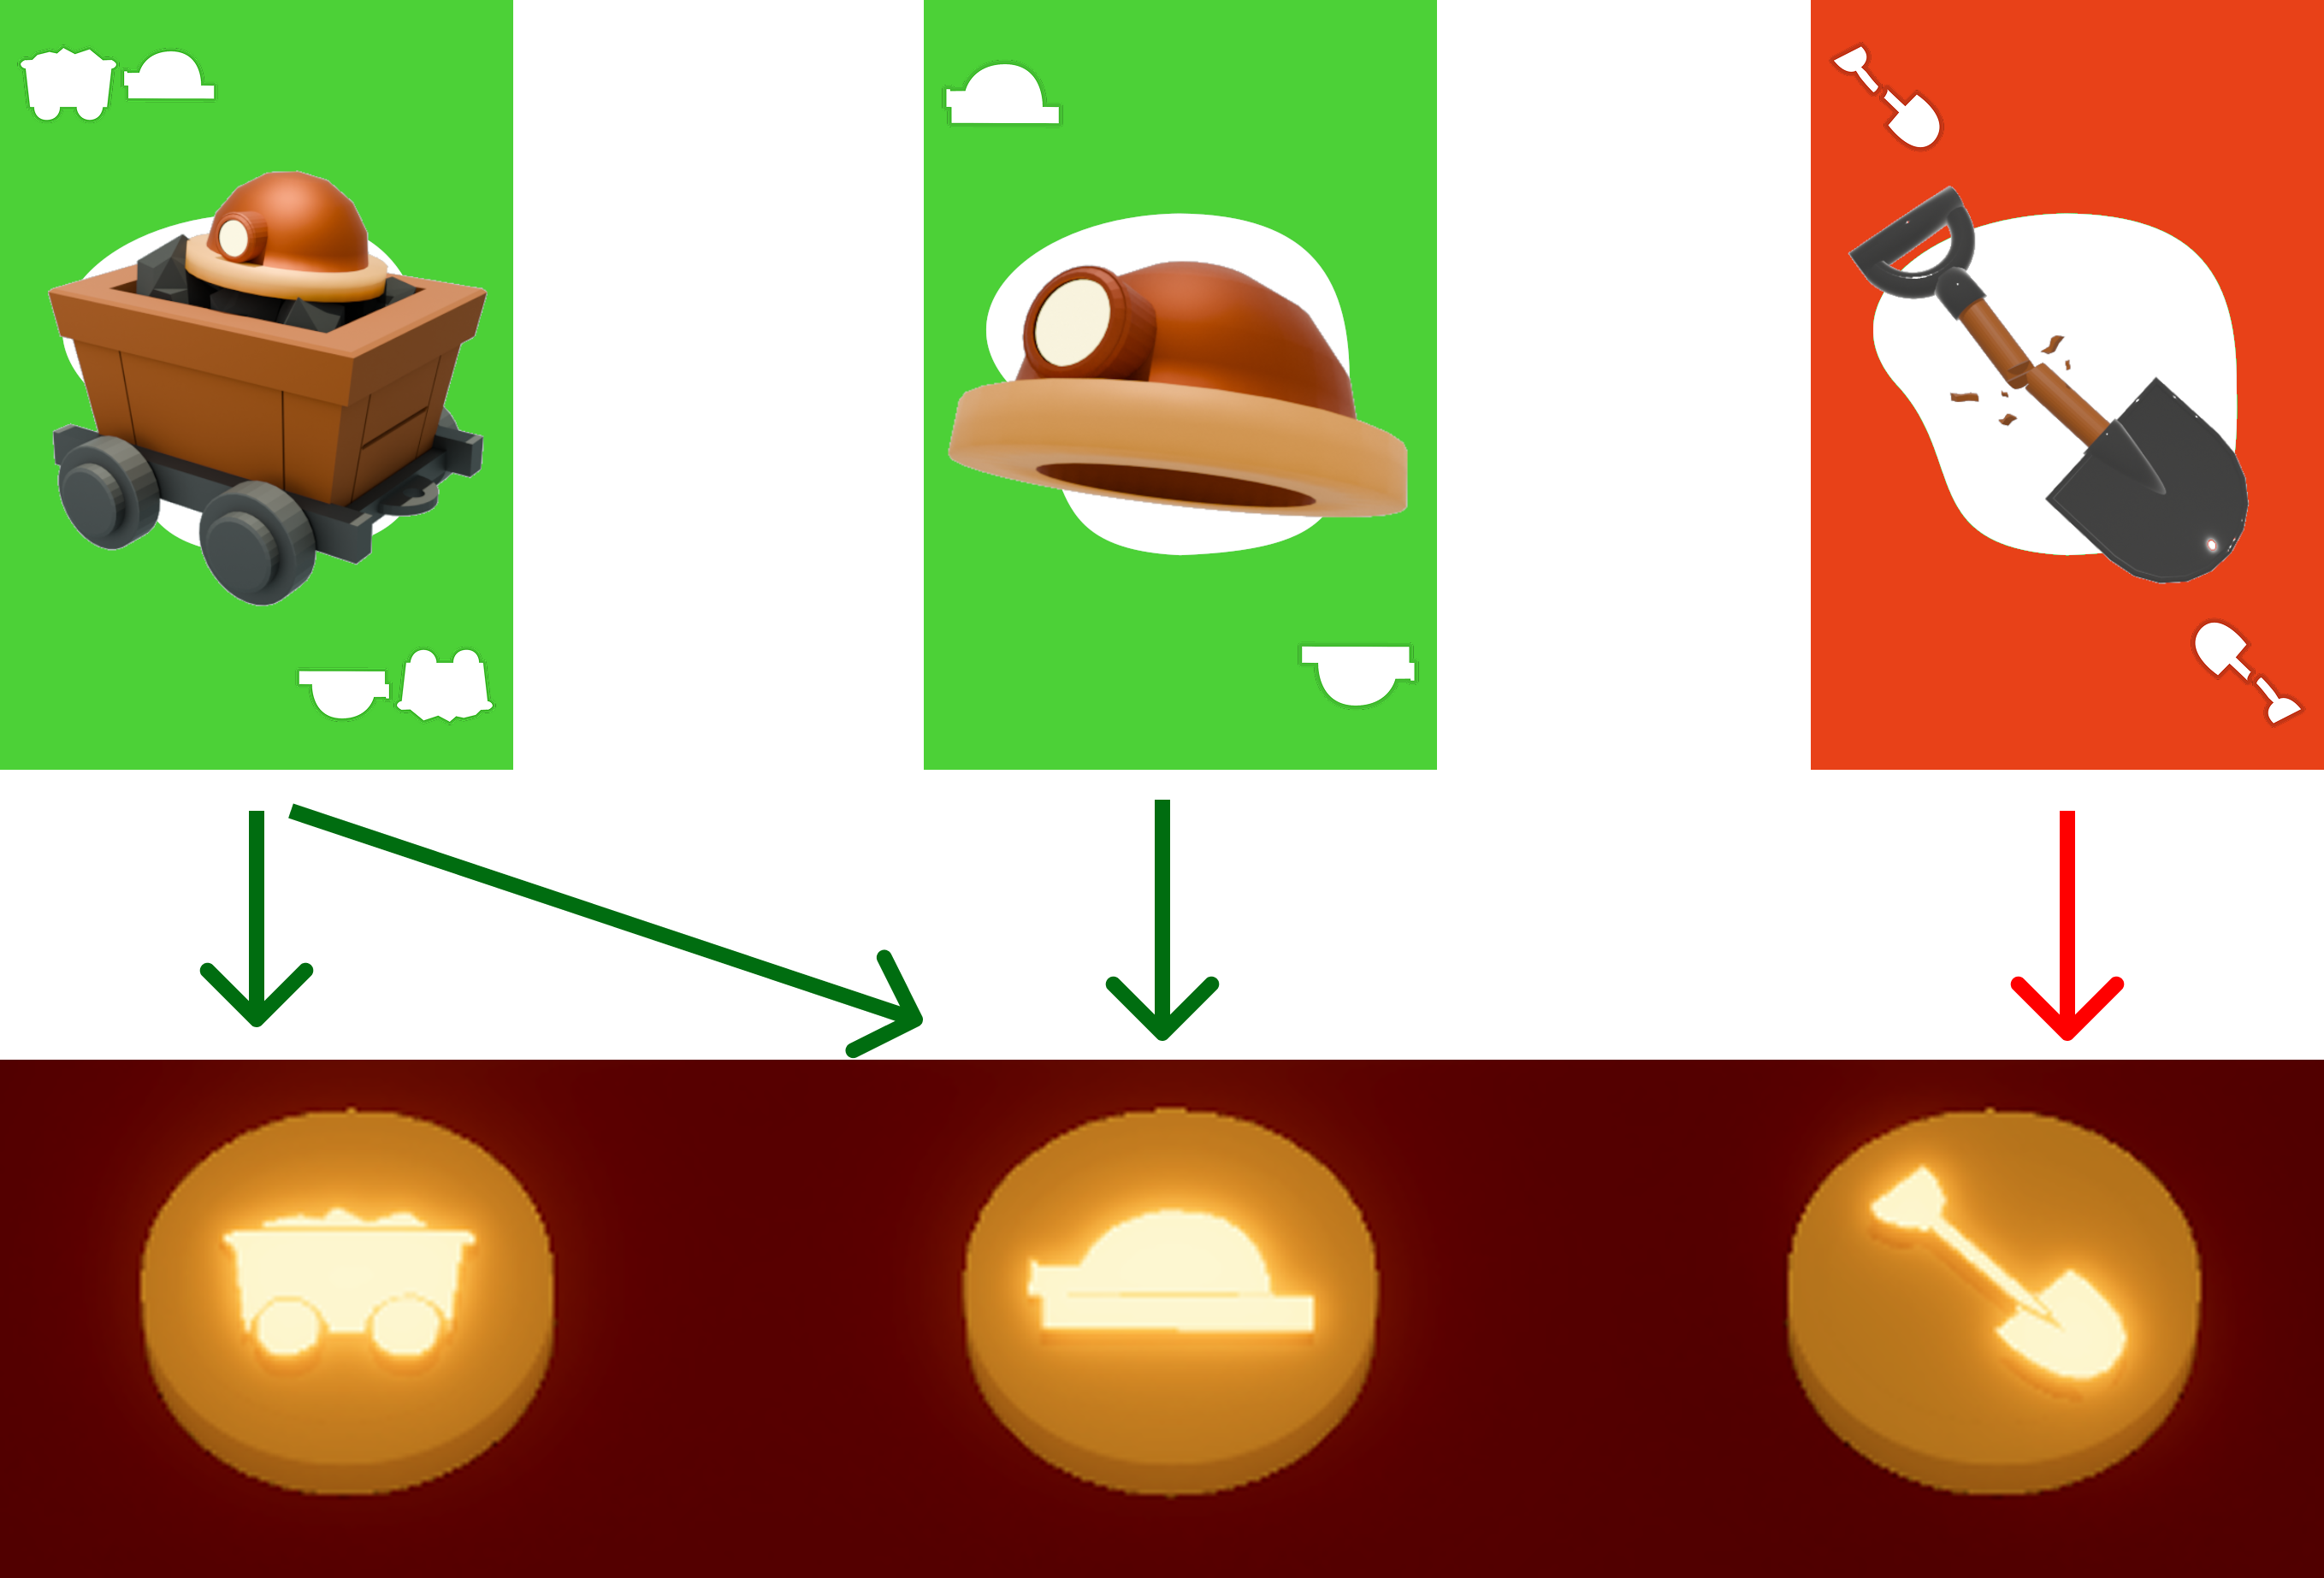
\includegraphics[width=0.5\linewidth]{saboteur/repair-n-break-cards.png}
        \caption*{Thẻ sửa và phá công cụ}
    \end{figure}
\end{frame}
% 10
\begin{frame}
\frametitle{Thẻ hành động (Action Cards)}
    \vspace{1cm}
    \begin{figure}[H]
        \centering
        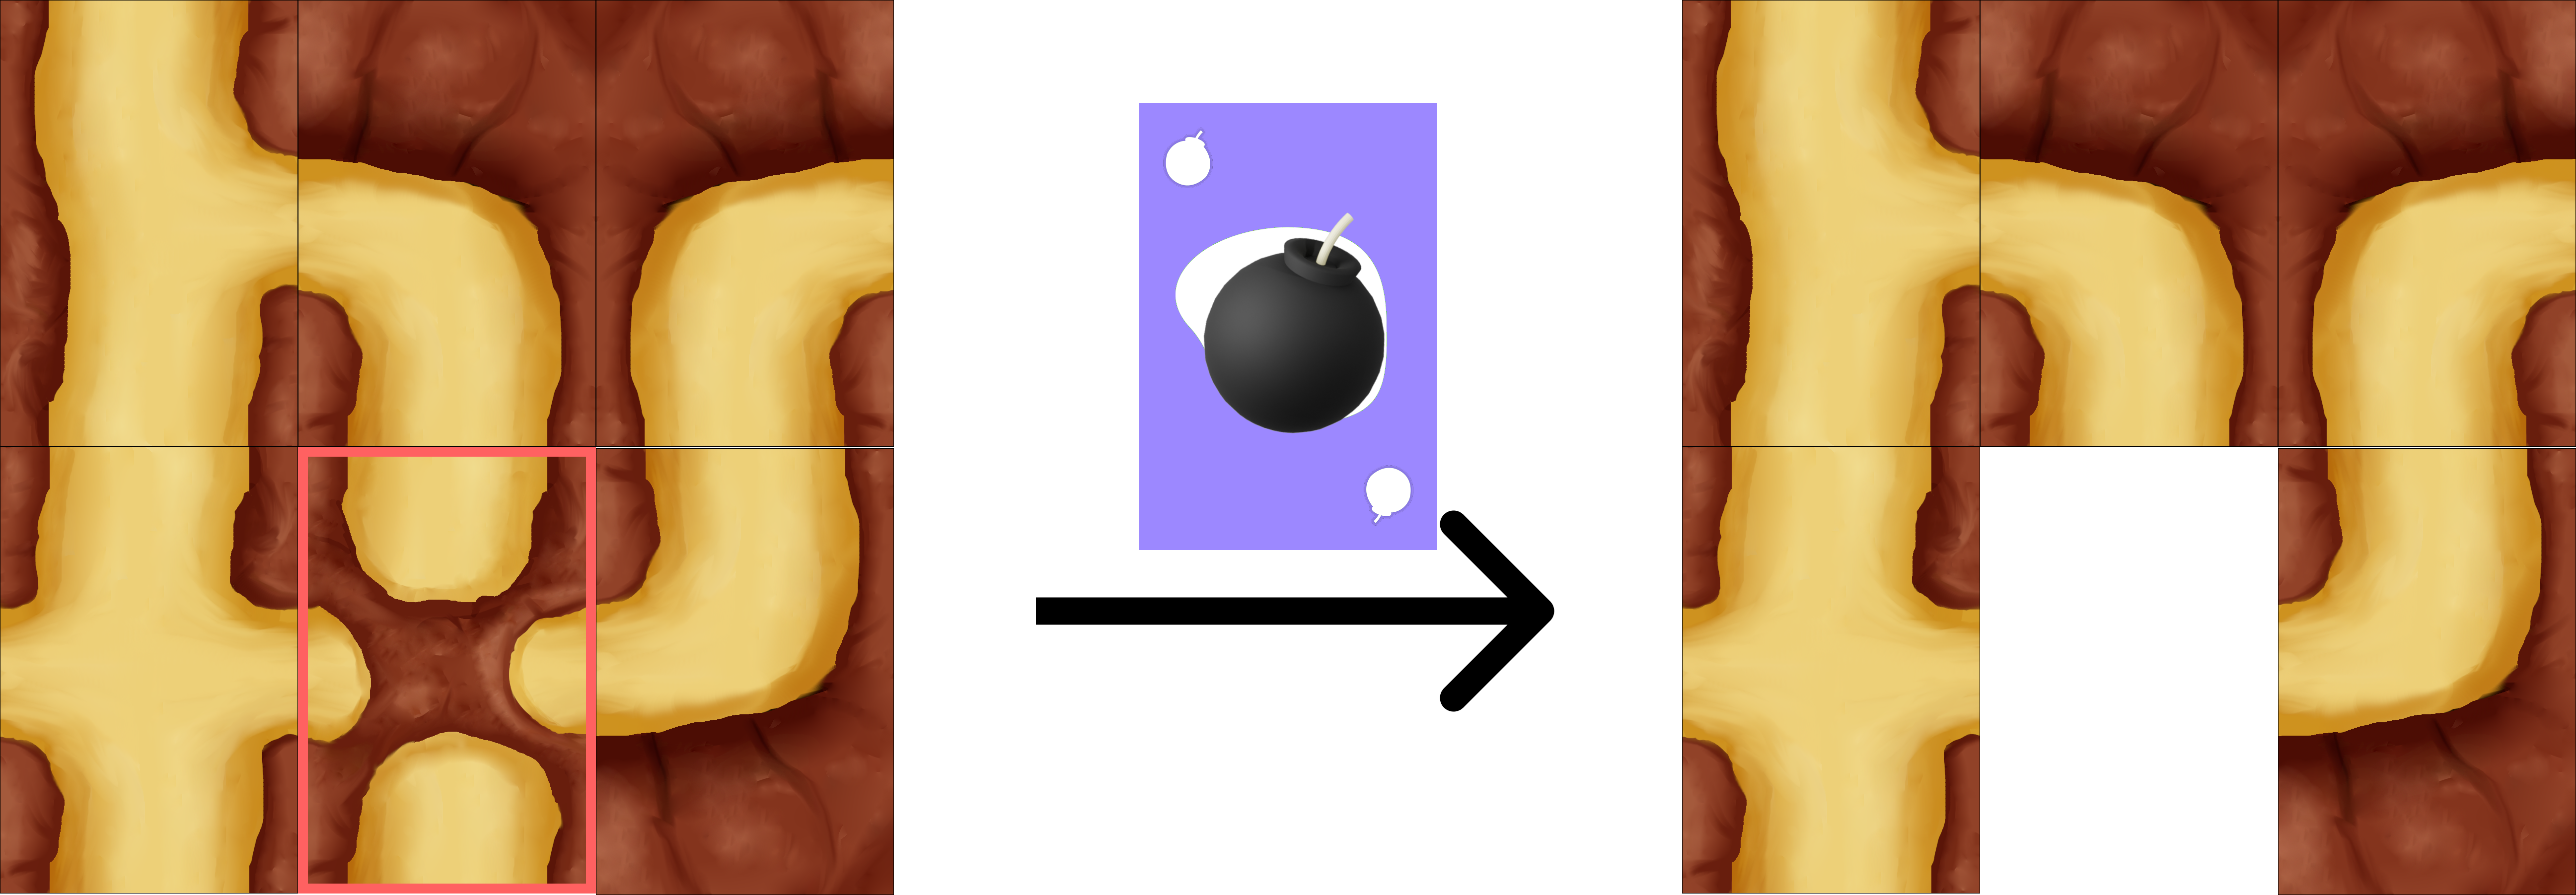
\includegraphics[width=0.6\linewidth]{saboteur/bomb-card.png}
        \caption*{Thẻ bomb}
    \end{figure}
\end{frame}

\begin{frame}
\frametitle{Thẻ hành động (Action Cards)}
    \vspace{1cm}
    \begin{figure}[H]
        \centering
        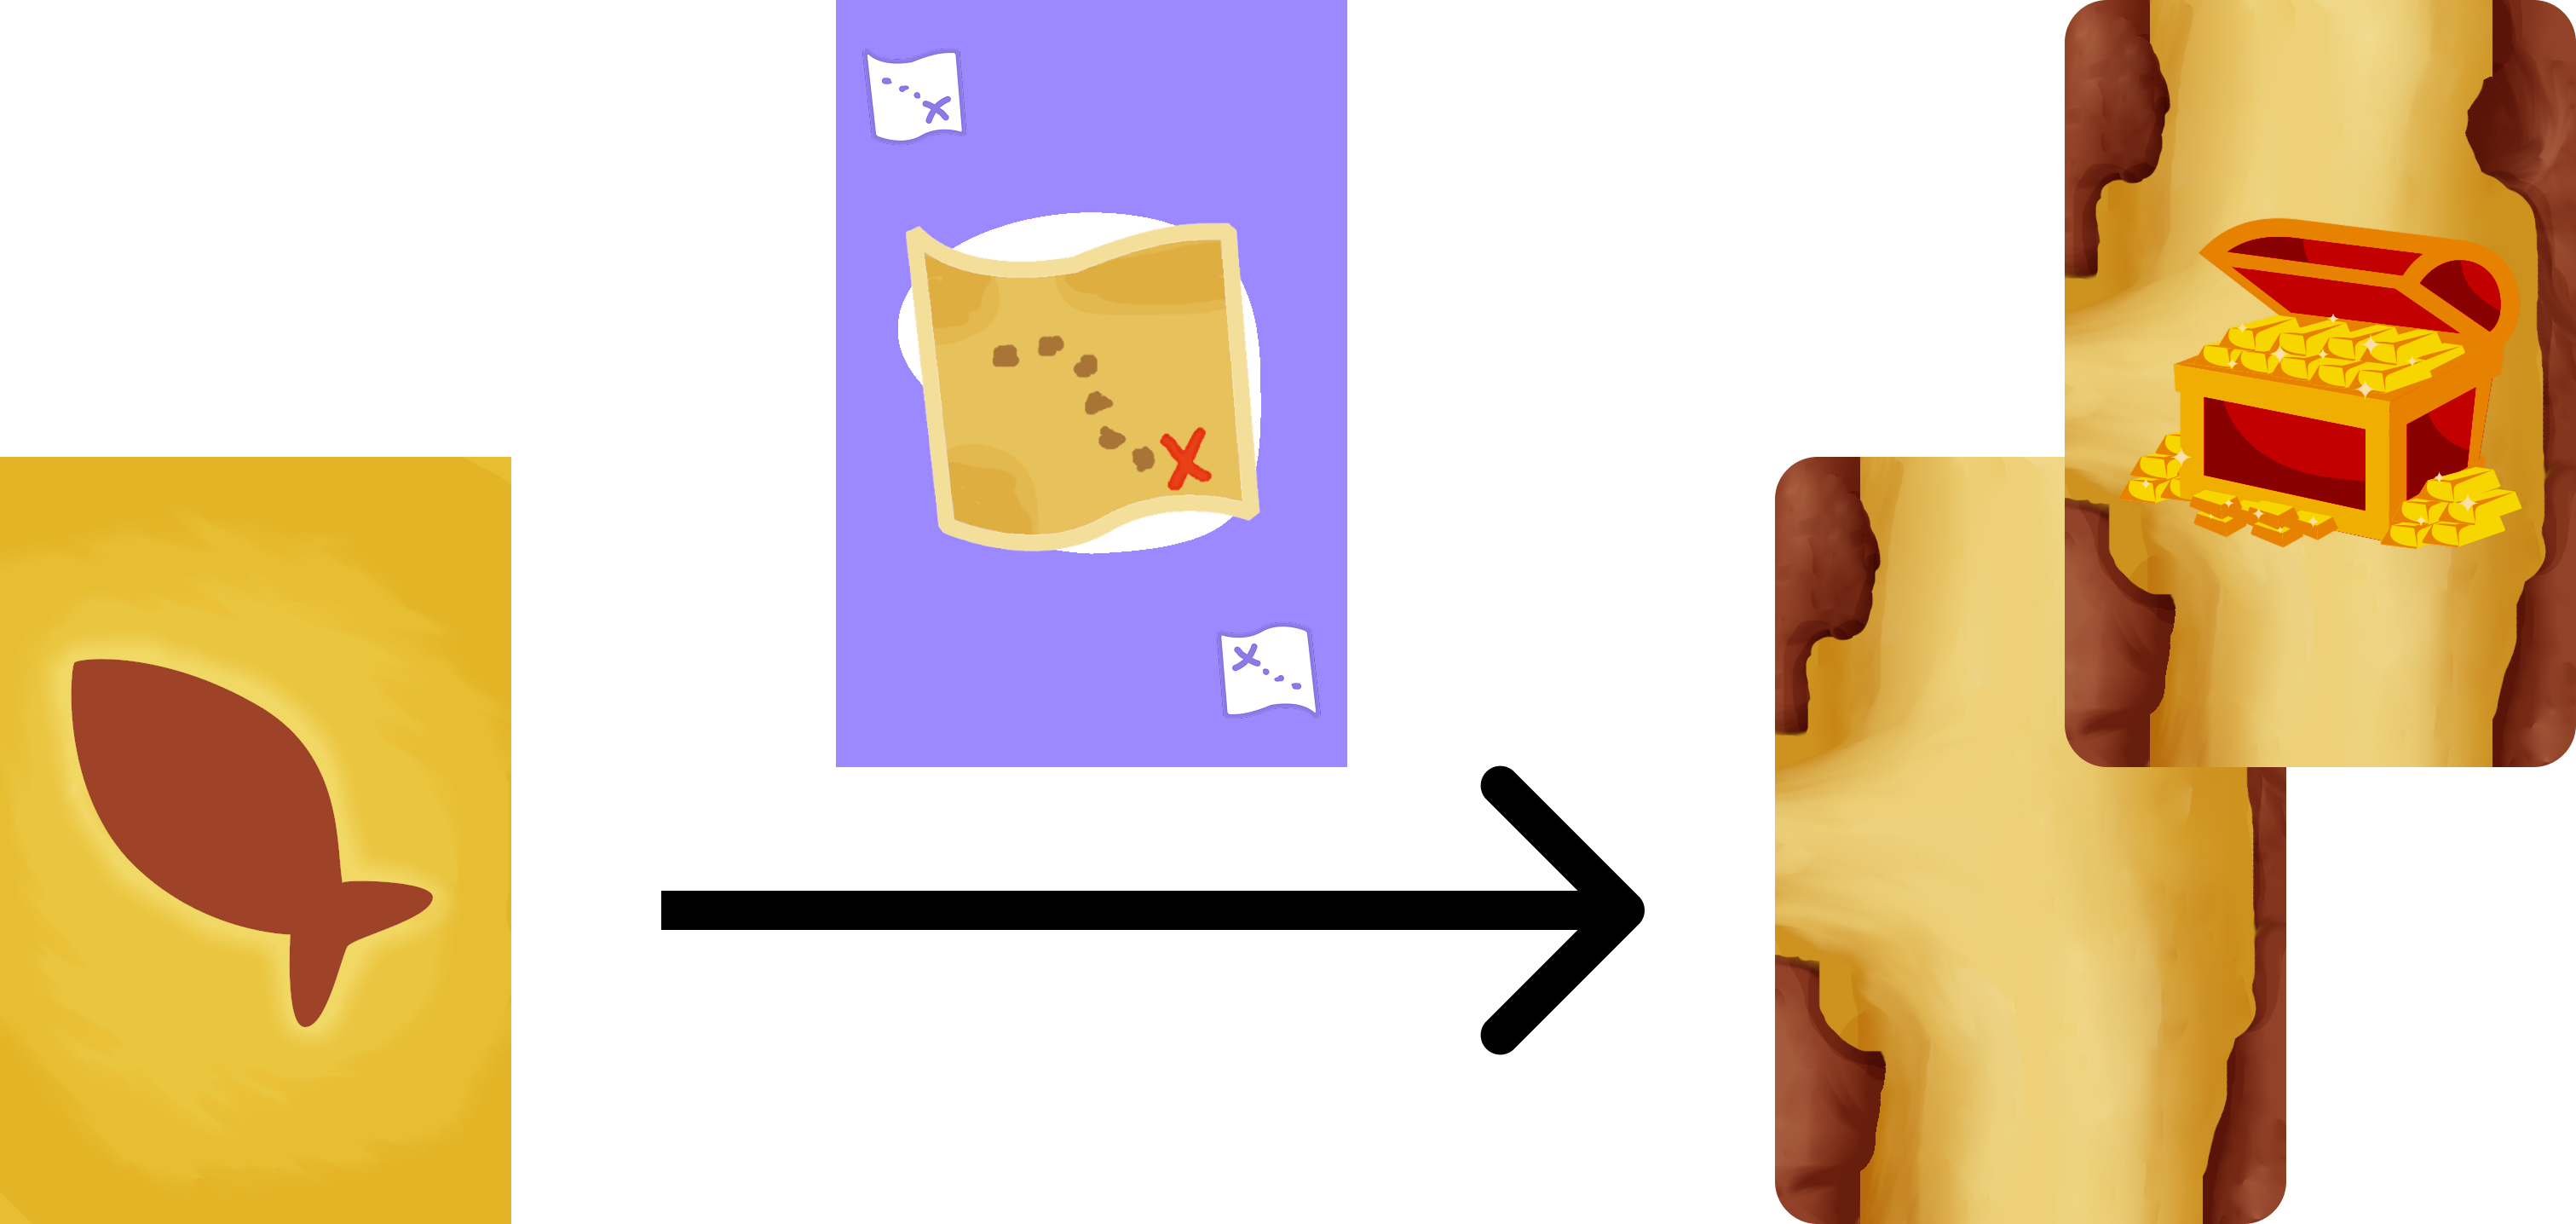
\includegraphics[width=0.5\linewidth]{saboteur/map-card.png}
        \caption*{Thẻ map}
    \end{figure}
\end{frame}



% New Saboteur
% 11
\begin{frame}
\frametitle{Sáng tạo luật chơi mới - Biến thể Saboteur với  ngày đêm}
    \begin{figure}[H]
        \centering
        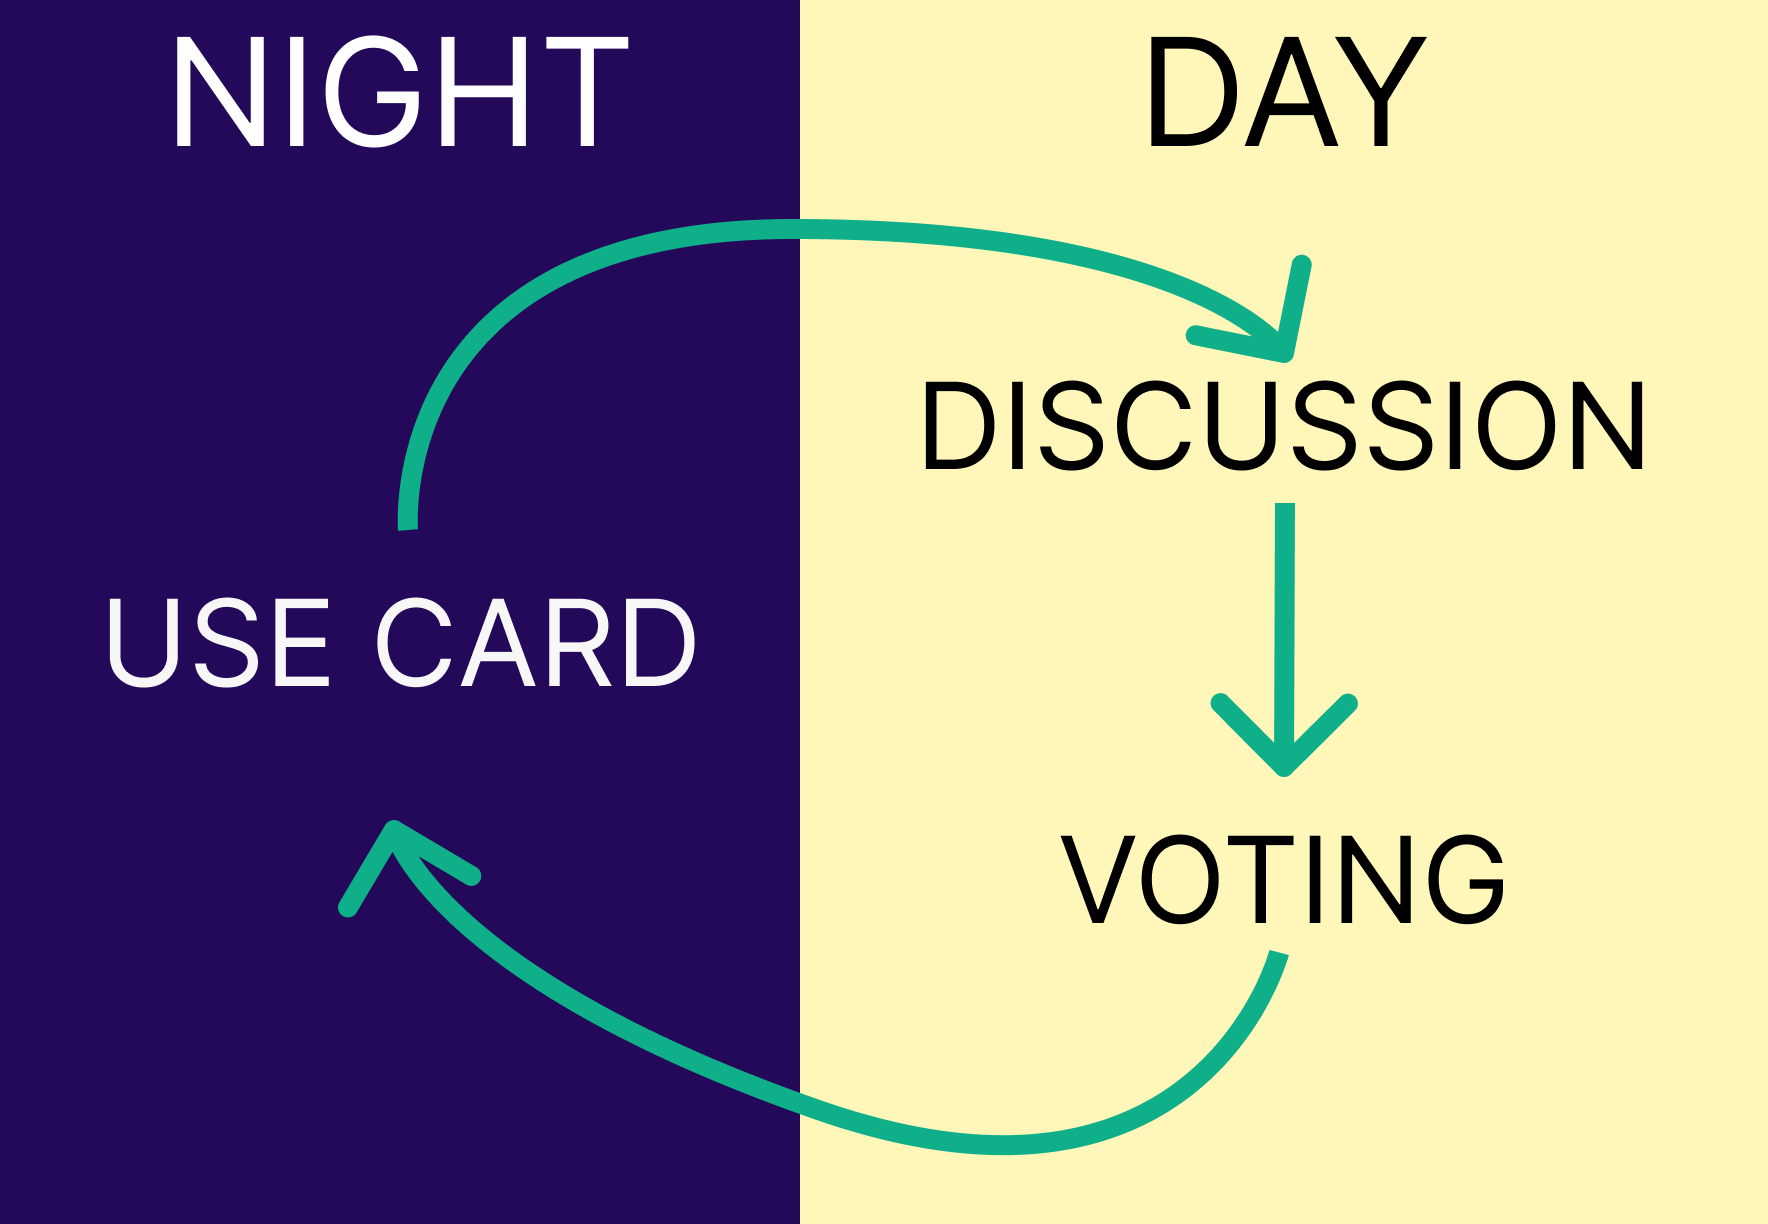
\includegraphics[width=0.5\linewidth]{saboteur/day-night.png}
    \end{figure}
Mỗi round được chia thành hai pha chính: \textbf{Đêm} và \textbf{Ngày}.
\end{frame}

% 12
\begin{frame}
\frametitle{Cấu trúc một round}

\textbf{Đêm (Night Phase):}
\begin{itemize}
    \item Màn hình/bản đồ tối lại, người chơi \textbf{không nhìn thấy bất kỳ thay đổi nào trên bản đồ} ngoại trừ thông tin lượt hiện tại.
    \item Thứ tự lượt chơi trong đêm được \textbf{xếp ngẫu nhiên} (không theo chiều kim đồng hồ như bản gốc).
    \item Mỗi người chơi lần lượt thực hiện lượt:
\begin{itemize}
    \item Bản đồ tạm thời hiện ra cho riêng người đó.
    \item Trong \textbf{15--30 giây} (có thể tùy chỉnh), người chơi thực hiện một trong các hành động quen thuộc như bản gốc.
    \item Bốc 1 lá bài từ chồng bài úp (nếu còn).
    \item Bản đồ lại tối đi với người chơi đó.
\end{itemize}
    \item Khi tất cả người chơi đã hoàn thành lượt trong đêm, pha Đêm kết thúc và chuyển sang pha Ngày.
\end{itemize}

\end{frame}

% 13
\begin{frame}
\frametitle{Cấu trúc một round}
\textbf{Ngày (Day Phase):}
    \begin{itemize}
        \item Bản đồ được chiếu sáng hoàn toàn, mọi người chơi cùng nhìn thấy toàn bộ thay đổi đã xảy ra trong pha Đêm.
        \item Người chơi có \textbf{60 giây} (có thể tùy chỉnh) để \textbf{trò chuyện, tranh luận, biện minh} và đọc vị nhau.
        \item Cuối pha Ngày, thực hiện \textbf{bỏ phiếu}:
        \begin{itemize}
            \item Có thể vote \textbf{skip} hoặc vote một người chơi cụ thể.
            \item Người bị vote nhiều phiếu nhất sẽ \textbf{không được hành động trong pha Đêm tiếp theo}.
        \end{itemize}
    \end{itemize}

\end{frame}

% 15
% \begin{frame}
% \frametitle{Thẻ hành động mới (bổ sung thêm vào bộ bài)}
% \begin{table}[H]
% \centering
% \begin{tabular}{|l|p{7cm}|p{4cm}|}
% \hline
% \textbf{Tên thẻ} & \textbf{Công dụng} & \textbf{Ghi chú} \\ \hline
% 
\includegraphics[width=0.1\linewidth]{saboteur/role-1.png} & Người chơi sẽ có khiên vĩnh viễn có thể đỡ được 1 đòn tấn công phá công cụ (Cart, Shovel, Hat) bởi thẻ Sabotage. & Có thể áp dụng cho bất cứ ai, không tích lũy \\ \hline
% Binoculars & Khi sử dụng thẻ này, người chơi được nhìn thấy toàn bộ bản đồ từ lúc chơi thẻ cho đến hết Đêm hiện tại. & Có thể áp dụng cho bất cứ ai\\ \hline
% Swap Goals & Trong Đêm, tráo vị trí ngẫu nhiên hoặc chỉ định của 3 thẻ Goal (khi chúng vẫn đang úp). & Thay đổi vị trí kho vàng thực sự \\ \hline
% \end{tabular}
% \end{table}
% \end{frame}

\begin{frame}
\frametitle{Thẻ hành động mới}
\begin{columns}
\column{0.33\textwidth}
    \begin{figure}[H]
        \centering
        
\includegraphics[width=0.4\linewidth]{saboteur/Card_Binoculars_S.png}
    \end{figure}
    \begin{itemize}
        \item Nhìn thấy toàn bộ bản đồ từ lúc chơi thẻ cho đến hết \textbf{Đêm} hiện tại.
    \end{itemize}
\column{0.33\textwidth}
    \begin{figure}[H]
        \centering
        
\includegraphics[width=0.4\linewidth]{saboteur/Card_Shield_S.png}
    \end{figure}
    \begin{itemize}
        \item Đỡ được 1 đòn tấn công phá công cụ. Không tích lũy
    \end{itemize}

\column{0.33\textwidth}
    \begin{figure}[H]
        \centering
        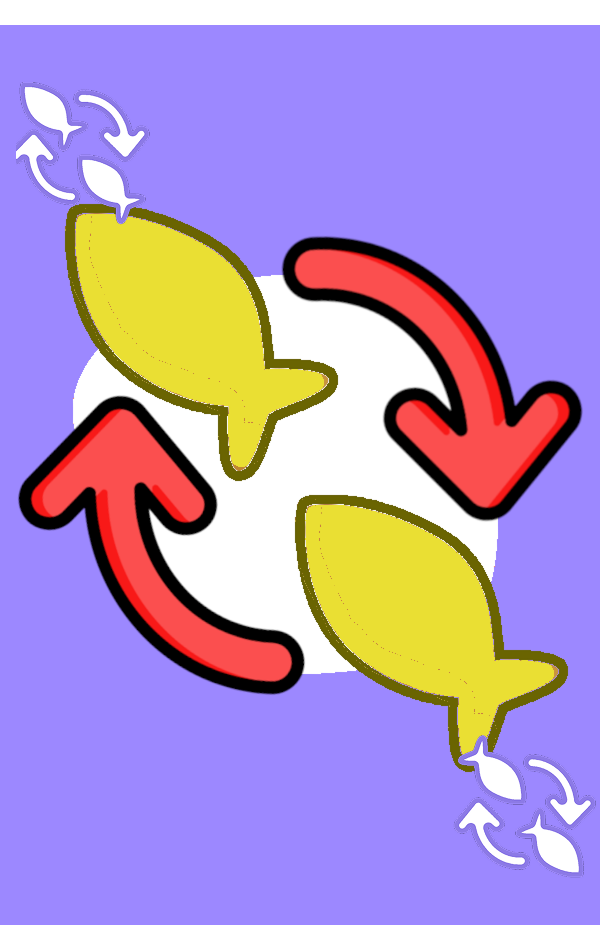
\includegraphics[width=0.4\linewidth]{saboteur/Card_Swap_Goals_S.png}
        % \caption*{Các loại thẻ đường}
    \end{figure}
    \begin{itemize}
        \item Hoán đổi vị trí của 2 trong 3 thẻ Goal (khi chúng vẫn đang úp)
    \end{itemize}
\end{columns}
\end{frame}